\subsection{Google Maps}
      \paragraph{}
	"Google Maps" est un service gratuit de cartographie en ligne. Le service a été créé par Google. 
	Lancé en 2004 aux États-Unis et au Canada et en 2005 en Grande-Bretagne (sous le nom de "Google Local"),
	Google Maps a été lancé jeudi 27 avril 2006, simultanément en France, Allemagne, Espagne et Italie \cite{T}.
      \paragraph{}
	Ce service permet, à partir de l'échelle d'un pays, de zoomer jusqu'à l'échelle d'une rue. Des prises 
	de vue fixes montrant les détails de certaines rues sont également accessibles grâce à une passerelle 
	vers "Google Street View" \footnote{ service lancé en mai 2007 afin de compléter "Google Maps" et "Google Earth": 
	Il permet de visualiser un panorama à 360° d'un lieu situé sur une voie urbaine ou rurale.}. Aussi il permet 
	de calculer des itinéraires, et de se renseigner par exemple sur les commerces 
	présents près de la position de l'utilisateur. 
      \paragraph{}
	Deux types de vue sont disponibles dans "Google Maps" : une vue en plan classique, avec les nom des villes, 
	des quartiers, des rues et une vue en image satellite, qui couvre aujourd'hui le monde entier.
      \paragraph{}
	Il existe également plusieurs versions mobiles de Google Maps, qui utilisent les réseaux des téléphones 
	notamment 3G pour charger les cartes de la même manière que sur les ordinateurs. Les versions varient 
	beaucoup selon la définition d'écran des téléphones portables, le fait d'avoir un écran tactile ou encore
	la puissance du processeur.
	
	  \begin{figure}[H]
	   \begin{center}
%	    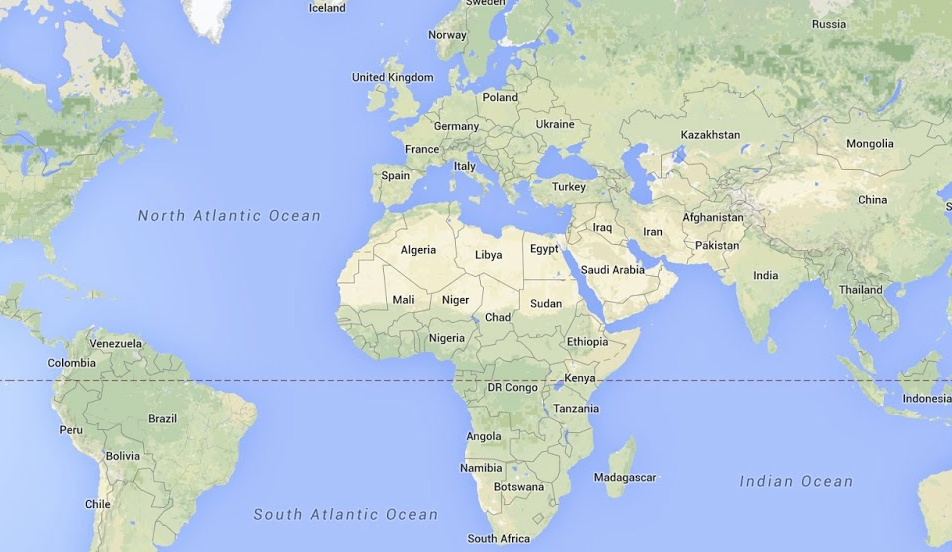
\includegraphics[scale=0.5]{images/carte_monde_ggm.png}
	    \caption[Carte du monde sous "Google Maps"]{Carte du monde sous "Google Maps" \protect \footnotemark}
	    \label{Carte du monde sous Google Maps}
	   \end{center}
	  \end{figure}
	  \footnotetext{Source:\url{www.google.bj/mapmaker}}

\subsection{OpenStreetMap}
      \paragraph{}
	"OpenStreetMap" (OSM) est un projet qui a pour but de constituer une base de données géographiques libre  (permettant par exemple de créer des cartes sous licence libre), en utilisant le système GPS et d'autres 
	données libres. Il a été initié en juillet 2004 par Steve Coast au University College de Londres \cite{U}. Il est mis à jour par l'utilisation de 
	moyens informatiques basés sur internet qui permettent l'intervention et la collaboration de tout utilisateur 
	volontaire.\\
	
      \paragraph{}
	Ce projet s'appuie donc sur les connaissances des collaborateurs, cela permettant notamment une mise à jour plus rapide 
	des données. "OpenStreetMap" peut être considéré comme le wikipédia de la cartographie libre.\\
	Il propose quasiment les mêmes services que Google Maps. Il faut aussi noter que les données d'OpenStreetMap
	sont gratuites pour les utilisations commerciales ce qui n'est pas le cas de "Google Maps".
	
      \paragraph{}
	Concernant le domaine du mobile il n'existe pas une application mobile nommée "OpenStreetMap" telle que celle de "Google Maps" mais
	 il existe plusieurs applications mobiles de cartographie qui utilisent les données d'OpenStreetMap telles que Osmand, OruxMaps
	 ou OSMTracker et bien d'autres \cite{V} qui permettent non seulement de profiter des services de géolocalisation mais aussi
	 d'ajouter des données cartographiques au serveur pour améliorer la carte.

      	  \begin{figure}[H]
	   \begin{center}
%	    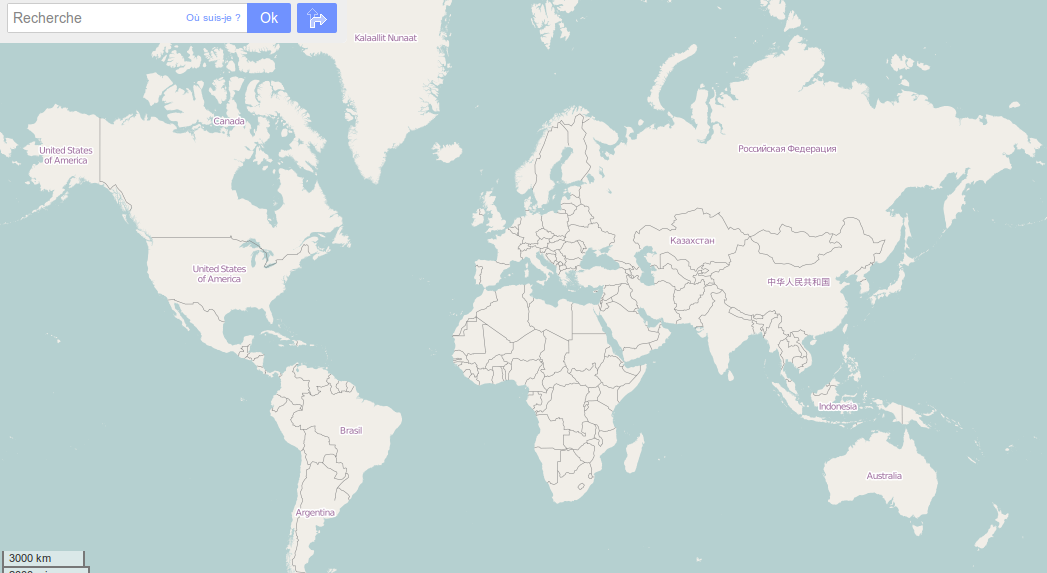
\includegraphics[scale=0.5]{images/carte_monde_osm.png}
	    \caption[Carte du monde sous "OpenStreetMap"]{Carte du monde sous "OpenStreetMap" \protect \footnotemark}
	    \label{Carte du monde sous OpenStreetMap}
	   \end{center}
	  \end{figure}
	  \footnotetext{Source:\url{www.openstreetmap.org}}
	  
	  
\section*{Conclusion}
	\paragraph{}
	  Les systèmes de géolocalisation constituent un outil d'aide très important pour faciliter et autonomiser les déplacements. Dans ce chapitre nous avons présenté leurs fonctionnements et quelques solutions existantes. Néanmoins ces solutions ne permettent
	  pas de résoudre le cas des déplacements à l'UAC car aucune d'elles ne présente la structure de celle-ci. Dans le chapitre suivant
	  nous aborderons notre solution à travers sa conception et les outils utilisés pour sa réalisation.